En regardant rapidement les données fournies dans le fichier \emph{train.txt}, on peut voir que les échanges de textos sont très courts. Également, il y a beaucoup d'\emph{emojis} et de binettes créés à partir de caractères spéciaux (ex: :), :D, :(, :-)).

On peut regarder le nombre de textes avec la présence d'au moins un emoji particulier selon chaque classe pour voir si ceux-ci semblent être beaucoup plus présents dans une classe ou une autre. Les résultats obtenus pour quelques emojis testés se trouvent dans la table \ref{table:emojis}

% Please add the following required packages to your document preamble:
% \usepackage{booktabs}
\begin{table}[]
	\centering
	\caption{Comptes préliminaires d'emojis}
	\label{table:emojis}
	\begin{tabular}{@{}lllll@{}}
		\toprule
		Emoji testé & Angry & Happy & Sad & Others \\ \midrule
		
\includegraphics[height=0.5cm]{images/heart}          & 8     & 31    & 13  & 41     \\
		
\includegraphics[height=0.3cm]{images/broken_heart}          & 2     & 0     & 64  & 3      \\
		
\includegraphics[height=0.3cm]{images/heart_eyes}          & 10    & 88    & 10  & 92     \\
		
\includegraphics[height=0.3cm]{images/sad}          & 15    & 1     & 282 & 15     \\
		
\includegraphics[height=0.3cm]{images/laughter}          & 59    & 989   & 49  & 197    \\
		
\includegraphics[height=0.3cm]{images/angry}          & 156   & 6     & 18  & 10     \\ \bottomrule
	\end{tabular}
\end{table}

%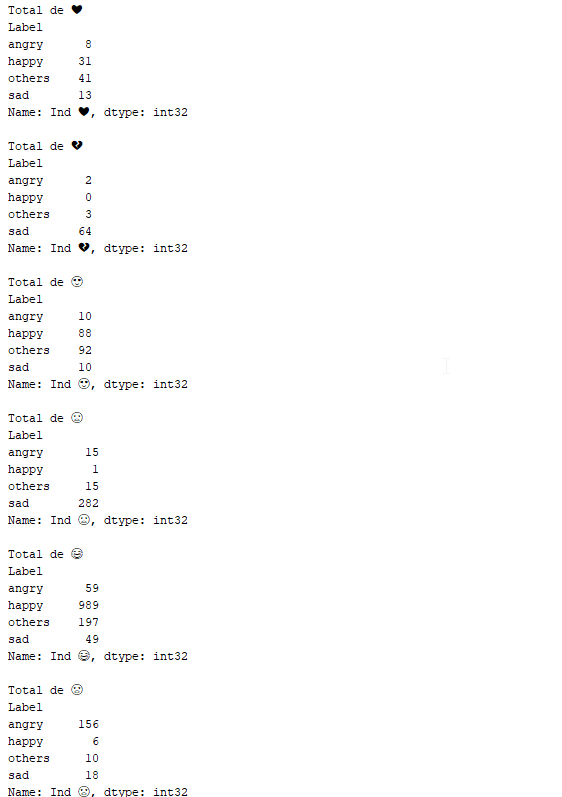
\includegraphics[width=\linewidth,height=15cm,keepaspectratio]{images/analyse_emojis}

À première vue, les emojis semblent avoir un impact important. Par exemple, le coeur brisé et le bonhomme triste sont souvent utilisés dans des échanges de textos tristes alors que celui qui fait un sourire est utilisé pour les échanges neutres ou joyeux. Il semble donc pertinent de convertir tous les emojis en texte pour les traiter avec un objet de compte de mots.

On peut également tenter de repérer les binettes créées à partir de caractères spéciaux. Pour parvenir à les identifier, on utilise une expression régulière qui identifie les séries de 2 à 6 caractères spéciaux. On voit ici ladite expression régulière avec la liste des chaînes de caractères ainsi extraites.
\begin{verbatim}
reg ex : [^\w\s\d]{2,6}
\end{verbatim}

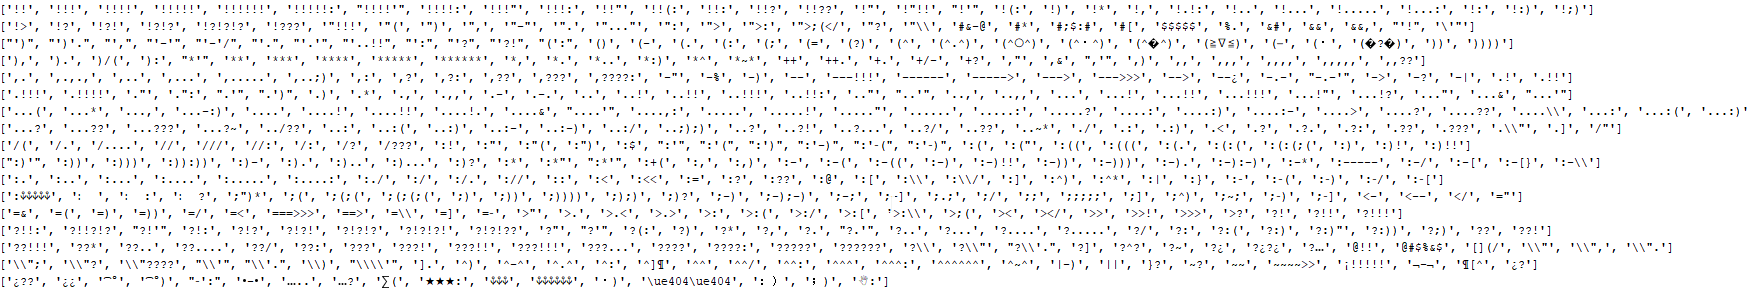
\includegraphics[width=\linewidth,height=7cm]{images/analyse_list_car_speciaux}

À partir de cela, on peut tenter d'identifier toutes les chaînes qui semblent intéressantes de façon manuelle. Pour voir rapidement si ces chaînes de caractères pourraient être discriminantes, on fait une analyse des comptes selon nos quatre classes. La table \ref{table:binettes} présente les résultats les plus intéressants.

% Please add the following required packages to your document preamble:
% \usepackage{booktabs}
% \usepackage{longtable}
% Note: It may be necessary to compile the document several times to get a multi-page table to line up properly
\begin{longtable}[c]{@{}lllll@{}}
	\caption{Comptes des chaînes de caractères spéciaux}
	\label{table:binettes}\\
	\toprule
	Chaîne de caractères & Angry & Happy & Sad & Others \\* \midrule
	\endhead
	%
	\bottomrule
	\endfoot
	%
	\endlastfoot
	%
	:)                   & 140   & 254   & 191 & 610    \\
	:D                   & 43    & 104   & 44  & 166    \\
	;)                   & 34    & 66    & 28  & 121    \\
	=)                   & 1     & 4     & 0   & 10     \\
	:-)                  & 22    & 50    & 27  & 74     \\
	;-)                  & 2     & 13    & 6   & 14     \\
	:(                   & 71    & 18    & 348 & 101    \\
	;(                   & 3     & 0     & 24  & 3      \\
	:'(                  & 7     & 3     & 29  & 6      \\
	:/                   & 40    & 13    & 33  & 49     \\
	:-/                  & 6     & 2     & 1   & 4      \\
	:-(                  & 5     & 0     & 21  & 6      \\
	Série de .           & 469   & 410   & 459 & 1085   \\
	Série de !           & 90    & 63    & 68  & 162    \\
	Série de ?           & 54    & 22    & 64  & 180    \\
	Série de ! ou ?      & 157   & 89    & 148 & 359    \\* \bottomrule
\end{longtable}

On peut voir que les smileys qui ont une apparence plus joyeuse (ex: :), :D) sont souvent utilisés dans des textos joyeux ou autres. Pour ce qui est de ceux avec une apparence triste, on remarque qu'ils sont souvent dans les textos tristes et parfois ceux fâchés.

On peut également analyser la ponctuation, plus particulièrement les séries de 3 signes de ponctuation et plus (ex: ..., !!!!!, ????, ?!?!??!). Les séries de points ne semblent pas se trouver en plus grande fréquence dans une classe en particulier. Pour ce qui est des séries de ! ou ?, on remarque qu'elles sont plus présentes dans les textos fâchés et tristes.

On peut également s'attarder au pourcentage de lettres en majuscule dans un texto, ainsi que le score de sentiment, le nombre de mots positifs et négatifs. Les résultats obtenus pour chacun de ces attributs sont présentés dans la table \ref{table:pourcentages}.

% Please add the following required packages to your document preamble:
% \usepackage{booktabs}
% \usepackage{longtable}
% Note: It may be necessary to compile the document several times to get a multi-page table to line up properly
\begin{longtable}[c]{@{}lllll@{}}
	\caption{Analyse des attributs de sentiments}
	\label{table:pourcentages}\\
	\toprule
	Attribut                           & Angry     & Happy    & Sad       & Others   \\* \midrule
	\endhead
	%
	\bottomrule
	\endfoot
	%
	\endlastfoot
	%
	Moyenne de lettres en majuscule    & 0,078271  & 0,079926 & 0,076783  & 0,082716 \\
	Moyenne de score de sentiment      & -0,272566 & 0,417544 & -0,201983 & 0,077257 \\
	Moyenne de nombre de mots positifs & 0,594987  & 1,181475 & 0,786198  & 0,698689 \\
	Moyenne de nombre de mots négatifs & 1,054668  & 0,538770 & 1,068094  & 0,523013 \\* \bottomrule
\end{longtable}


%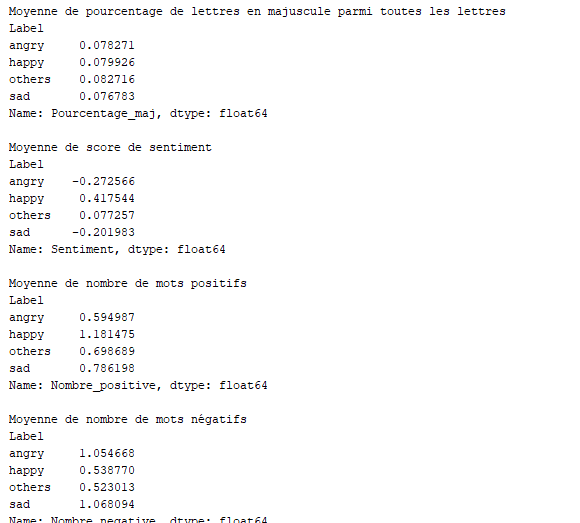
\includegraphics[width=\linewidth,height=15cm,keepaspectratio]{images/analyse_maj_sentiment}

Le score de sentiment utilisé est calculé avec \emph{Senti Word Net} en sommant les valeurs de sentiment attribuées à chaque mot de l'échange de textos. Le nombre de mots positifs/négatifs est calculé en comptant le nombre de mots avec des valeurs de sentiment supérieur/inférieur à 0.

On constate que le pourcentage de lettre majuscules dans les textos est similaire pour toutes les classes. On aurait pu penser que cette mesure aurait été plus élevée pour les textos fâchés, mais ça ne semble pas être le cas. 

Les 3 variables associées aux sentiments semblent beaucoup parler. En effet, les catégories triste et fâché ont des connotations beaucoup plus négatives, alors que la classe joyeuse a beaucoup plus de mots positifs. La classe \emph{Others} quand à elle a un score presque égal à 0. Ces résultats confirment notre intuition quant à l'utilisation de cet attribut.
